\documentclass[1p]{elsarticle_modified}
%\bibliographystyle{elsarticle-num}

%\usepackage[colorlinks]{hyperref}
%\usepackage{abbrmath_seonhwa} %\Abb, \Ascr, \Acal ,\Abf, \Afrak
\usepackage{amsfonts}
\usepackage{amssymb}
\usepackage{amsmath}
\usepackage{amsthm}
\usepackage{scalefnt}
\usepackage{amsbsy}
\usepackage{kotex}
\usepackage{caption}
\usepackage{subfig}
\usepackage{color}
\usepackage{graphicx}
\usepackage{xcolor} %% white, black, red, green, blue, cyan, magenta, yellow
\usepackage{float}
\usepackage{setspace}
\usepackage{hyperref}

\usepackage{tikz}
\usetikzlibrary{arrows}

\usepackage{multirow}
\usepackage{array} % fixed length table
\usepackage{hhline}

%%%%%%%%%%%%%%%%%%%%%
\makeatletter
\renewcommand*\env@matrix[1][\arraystretch]{%
	\edef\arraystretch{#1}%
	\hskip -\arraycolsep
	\let\@ifnextchar\new@ifnextchar
	\array{*\c@MaxMatrixCols c}}
\makeatother %https://tex.stackexchange.com/questions/14071/how-can-i-increase-the-line-spacing-in-a-matrix
%%%%%%%%%%%%%%%

\usepackage[normalem]{ulem}

\newcommand{\msout}[1]{\ifmmode\text{\sout{\ensuremath{#1}}}\else\sout{#1}\fi}
%SOURCE: \msout is \stkout macro in https://tex.stackexchange.com/questions/20609/strikeout-in-math-mode

\newcommand{\cancel}[1]{
	\ifmmode
	{\color{red}\msout{#1}}
	\else
	{\color{red}\sout{#1}}
	\fi
}

\newcommand{\add}[1]{
	{\color{blue}\uwave{#1}}
}

\newcommand{\replace}[2]{
	\ifmmode
	{\color{red}\msout{#1}}{\color{blue}\uwave{#2}}
	\else
	{\color{red}\sout{#1}}{\color{blue}\uwave{#2}}
	\fi
}

\newcommand{\Sol}{\mathcal{S}} %segment
\newcommand{\D}{D} %diagram
\newcommand{\A}{\mathcal{A}} %arc


%%%%%%%%%%%%%%%%%%%%%%%%%%%%%5 test

\def\sl{\operatorname{\textup{SL}}(2,\Cbb)}
\def\psl{\operatorname{\textup{PSL}}(2,\Cbb)}
\def\quan{\mkern 1mu \triangleright \mkern 1mu}

\theoremstyle{definition}
\newtheorem{thm}{Theorem}[section]
\newtheorem{prop}[thm]{Proposition}
\newtheorem{lem}[thm]{Lemma}
\newtheorem{ques}[thm]{Question}
\newtheorem{cor}[thm]{Corollary}
\newtheorem{defn}[thm]{Definition}
\newtheorem{exam}[thm]{Example}
\newtheorem{rmk}[thm]{Remark}
\newtheorem{alg}[thm]{Algorithm}

\newcommand{\I}{\sqrt{-1}}
\begin{document}

%\begin{frontmatter}
%
%\title{Boundary parabolic representations of knots up to 8 crossings}
%
%%% Group authors per affiliation:
%\author{Yunhi Cho} 
%\address{Department of Mathematics, University of Seoul, Seoul, Korea}
%\ead{yhcho@uos.ac.kr}
%
%
%\author{Seonhwa Kim} %\fnref{s_kim}}
%\address{Center for Geometry and Physics, Institute for Basic Science, Pohang, 37673, Korea}
%\ead{ryeona17@ibs.re.kr}
%
%\author{Hyuk Kim}
%\address{Department of Mathematical Sciences, Seoul National University, Seoul 08826, Korea}
%\ead{hyukkim@snu.ac.kr}
%
%\author{Seokbeom Yoon}
%\address{Department of Mathematical Sciences, Seoul National University, Seoul, 08826,  Korea}
%\ead{sbyoon15@snu.ac.kr}
%
%\begin{abstract}
%We find all boundary parabolic representation of knots up to 8 crossings.
%
%\end{abstract}
%\begin{keyword}
%    \MSC[2010] 57M25 
%\end{keyword}
%
%\end{frontmatter}

%\linenumbers
%\tableofcontents
%
\newcommand\colored[1]{\textcolor{white}{\rule[-0.35ex]{0.8em}{1.4ex}}\kern-0.8em\color{red} #1}%
%\newcommand\colored[1]{\textcolor{white}{ #1}\kern-2.17ex	\textcolor{white}{ #1}\kern-1.81ex	\textcolor{white}{ #1}\kern-2.15ex\color{red}#1	}

{\Large $\underline{11n_{9}~(K11n_{9})}$}

\setlength{\tabcolsep}{10pt}
\renewcommand{\arraystretch}{1.6}
\vspace{1cm}\begin{tabular}{m{100pt}>{\centering\arraybackslash}m{274pt}}
\multirow{5}{120pt}{
	\centering
	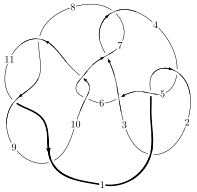
\includegraphics[width=112pt]{../../../GIT/diagram.site/Diagrams/png/625_11n_9.png}\\
\ \ \ A knot diagram\footnotemark}&
\allowdisplaybreaks
\textbf{Linearized knot diagam} \\
\cline{2-2}
 &
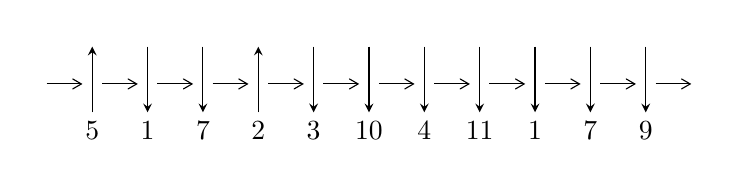
\begin{tikzpicture}[x=20pt, y=17pt]
	% nodes
	\node (C0) at (0, 0) {};
	\node (C1) at (1, 0) {};
	\node (C1U) at (1, +1) {};
	\node (C1D) at (1, -1) {5};

	\node (C2) at (2, 0) {};
	\node (C2U) at (2, +1) {};
	\node (C2D) at (2, -1) {1};

	\node (C3) at (3, 0) {};
	\node (C3U) at (3, +1) {};
	\node (C3D) at (3, -1) {7};

	\node (C4) at (4, 0) {};
	\node (C4U) at (4, +1) {};
	\node (C4D) at (4, -1) {2};

	\node (C5) at (5, 0) {};
	\node (C5U) at (5, +1) {};
	\node (C5D) at (5, -1) {3};

	\node (C6) at (6, 0) {};
	\node (C6U) at (6, +1) {};
	\node (C6D) at (6, -1) {10};

	\node (C7) at (7, 0) {};
	\node (C7U) at (7, +1) {};
	\node (C7D) at (7, -1) {4};

	\node (C8) at (8, 0) {};
	\node (C8U) at (8, +1) {};
	\node (C8D) at (8, -1) {11};

	\node (C9) at (9, 0) {};
	\node (C9U) at (9, +1) {};
	\node (C9D) at (9, -1) {1};

	\node (C10) at (10, 0) {};
	\node (C10U) at (10, +1) {};
	\node (C10D) at (10, -1) {7};

	\node (C11) at (11, 0) {};
	\node (C11U) at (11, +1) {};
	\node (C11D) at (11, -1) {9};
	\node (C12) at (12, 0) {};

	% arrows
	\draw[->,>={angle 60}]
	(C0) edge (C1) (C1) edge (C2) (C2) edge (C3) (C3) edge (C4) (C4) edge (C5) (C5) edge (C6) (C6) edge (C7) (C7) edge (C8) (C8) edge (C9) (C9) edge (C10) (C10) edge (C11) (C11) edge (C12) ;	\draw[->,>=stealth]
	(C1D) edge (C1U) (C2U) edge (C2D) (C3U) edge (C3D) (C4D) edge (C4U) (C5U) edge (C5D) (C6U) edge (C6D) (C7U) edge (C7D) (C8U) edge (C8D) (C9U) edge (C9D) (C10U) edge (C10D) (C11U) edge (C11D) ;
	\end{tikzpicture} \\
\hhline{~~} \\& 
\textbf{Solving Sequence} \\ \cline{2-2} 
 &
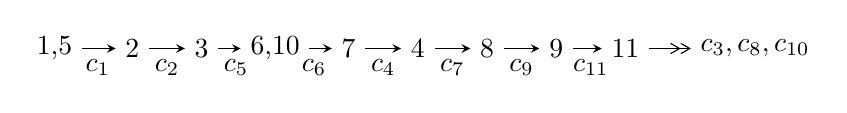
\begin{tikzpicture}[x=25pt, y=7pt]
	% node
	\node (A0) at (-1/8, 0) {1,5};
	\node (A1) at (1, 0) {2};
	\node (A2) at (2, 0) {3};
	\node (A3) at (49/16, 0) {6,10};
	\node (A4) at (33/8, 0) {7};
	\node (A5) at (41/8, 0) {4};
	\node (A6) at (49/8, 0) {8};
	\node (A7) at (57/8, 0) {9};
	\node (A8) at (65/8, 0) {11};
	\node (C1) at (1/2, -1) {$c_{1}$};
	\node (C2) at (3/2, -1) {$c_{2}$};
	\node (C3) at (5/2, -1) {$c_{5}$};
	\node (C4) at (29/8, -1) {$c_{6}$};
	\node (C5) at (37/8, -1) {$c_{4}$};
	\node (C6) at (45/8, -1) {$c_{7}$};
	\node (C7) at (53/8, -1) {$c_{9}$};
	\node (C8) at (61/8, -1) {$c_{11}$};
	\node (A9) at (10, 0) {$c_{3},c_{8},c_{10}$};

	% edge
	\draw[->,>=stealth]	
	(A0) edge (A1) (A1) edge (A2) (A2) edge (A3) (A3) edge (A4) (A4) edge (A5) (A5) edge (A6) (A6) edge (A7) (A7) edge (A8) ;
	\draw[->>,>={angle 60}]	
	(A8) edge (A9);
\end{tikzpicture} \\ 

\end{tabular} \\

\footnotetext{
The image of knot diagram is generated by the software ``\textbf{Draw programme}" developed by Andrew Bartholomew(\url{http://www.layer8.co.uk/maths/draw/index.htm\#Running-draw}), where we modified some parts for our purpose(\url{https://github.com/CATsTAILs/LinksPainter}).
}\phantom \\ \newline 
\centering \textbf{Ideals for irreducible components\footnotemark of $X_{\text{par}}$} 
 
\begin{align*}
I^u_{1}&=\langle 
7 u^{10}-25 u^9+49 u^8-40 u^7+18 u^6-11 u^5+35 u^4+u^2+46 b-21 u+24,\\
\phantom{I^u_{1}}&\phantom{= \langle  }-31 u^{10}+114 u^9-240 u^8+279 u^7-290 u^6+305 u^5-408 u^4+253 u^3-241 u^2+46 a+116 u-241,\\
\phantom{I^u_{1}}&\phantom{= \langle  }u^{11}-4 u^{10}+9 u^9-12 u^8+13 u^7-13 u^6+16 u^5-12 u^4+10 u^3-4 u^2+8 u-1\rangle \\
I^u_{2}&=\langle 
b+1,\;- u^4+u^3-2 u^2+a+u-1,\;u^5- u^4+2 u^3- u^2+u-1\rangle \\
I^u_{3}&=\langle 
- a u+3 b+a+u-1,\;a^2+a u-4 u-4,\;u^2+u+1\rangle \\
\\
\end{align*}
\raggedright * 3 irreducible components of $\dim_{\mathbb{C}}=0$, with total 20 representations.\\
\footnotetext{All coefficients of polynomials are rational numbers. But the coefficients are sometimes approximated in decimal forms when there is not enough margin.}
\newpage
\renewcommand{\arraystretch}{1}
\centering \section*{I. $I^u_{1}= \langle 7 u^{10}-25 u^9+\cdots+46 b+24,\;-31 u^{10}+114 u^9+\cdots+46 a-241,\;u^{11}-4 u^{10}+\cdots+8 u-1 \rangle$}
\flushleft \textbf{(i) Arc colorings}\\
\begin{tabular}{m{7pt} m{180pt} m{7pt} m{180pt} }
\flushright $a_{1}=$&$\begin{pmatrix}1\\0\end{pmatrix}$ \\
\flushright $a_{5}=$&$\begin{pmatrix}0\\u\end{pmatrix}$ \\
\flushright $a_{2}=$&$\begin{pmatrix}1\\- u^2\end{pmatrix}$ \\
\flushright $a_{3}=$&$\begin{pmatrix}u^2+1\\- u^2\end{pmatrix}$ \\
\flushright $a_{6}=$&$\begin{pmatrix}- u^5-2 u^3- u\\u^5+u^3+u\end{pmatrix}$ \\
\flushright $a_{10}=$&$\begin{pmatrix}0.673913 u^{10}-2.47826 u^{9}+\cdots-2.52174 u+5.23913\\-0.152174 u^{10}+0.543478 u^{9}+\cdots+0.456522 u-0.521739\end{pmatrix}$ \\
\flushright $a_{7}=$&$\begin{pmatrix}-0.173913 u^{10}+0.978261 u^{9}+\cdots+1.02174 u-3.23913\\-0.282609 u^{10}+1.15217 u^{9}+\cdots+1.84783 u+0.173913\end{pmatrix}$ \\
\flushright $a_{4}=$&$\begin{pmatrix}- u\\u^3+u\end{pmatrix}$ \\
\flushright $a_{8}=$&$\begin{pmatrix}0.260870 u^{10}-0.717391 u^{9}+\cdots-1.28261 u-2.89130\\-0.0217391 u^{10}+0.934783 u^{9}+\cdots+4.06522 u-0.217391\end{pmatrix}$ \\
\flushright $a_{9}=$&$\begin{pmatrix}0.521739 u^{10}-1.93478 u^{9}+\cdots-2.06522 u+4.71739\\-0.152174 u^{10}+0.543478 u^{9}+\cdots+0.456522 u-0.521739\end{pmatrix}$ \\
\flushright $a_{11}=$&$\begin{pmatrix}0.0652174 u^{10}-0.304348 u^{9}+\cdots-0.695652 u+3.15217\\0.108696 u^{10}-0.673913 u^{9}+\cdots-2.32609 u+0.0869565\end{pmatrix}$\\ \flushright $a_{11}=$&$\begin{pmatrix}0.0652174 u^{10}-0.304348 u^{9}+\cdots-0.695652 u+3.15217\\0.108696 u^{10}-0.673913 u^{9}+\cdots-2.32609 u+0.0869565\end{pmatrix}$\\&\end{tabular}
\flushleft \textbf{(ii) Obstruction class $= -1$}\\~\\
\flushleft \textbf{(iii) Cusp Shapes $= -\frac{13}{46} u^{10}+\frac{53}{46} u^9-\frac{137}{46} u^8+\frac{93}{23} u^7-\frac{89}{23} u^6+\frac{119}{46} u^5-\frac{203}{46} u^4+6 u^3-\frac{337}{46} u^2+\frac{39}{46} u-\frac{272}{23}$}\\~\\
\newpage\renewcommand{\arraystretch}{1}
\flushleft \textbf{(iv) u-Polynomials at the component}\newline \\
\begin{tabular}{m{50pt}|m{274pt}}
Crossings & \hspace{64pt}u-Polynomials at each crossing \\
\hline $$\begin{aligned}c_{1},c_{4}\end{aligned}$$&$\begin{aligned}
&u^{11}+4 u^{10}+\cdots+8 u+1
\end{aligned}$\\
\hline $$\begin{aligned}c_{2}\end{aligned}$$&$\begin{aligned}
&u^{11}+2 u^{10}+\cdots+56 u-1
\end{aligned}$\\
\hline $$\begin{aligned}c_{3},c_{7}\end{aligned}$$&$\begin{aligned}
&u^{11}-3 u^{10}+\cdots+16 u+16
\end{aligned}$\\
\hline $$\begin{aligned}c_{5}\end{aligned}$$&$\begin{aligned}
&u^{11}-4 u^{10}+\cdots+790 u+97
\end{aligned}$\\
\hline $$\begin{aligned}c_{6},c_{10}\end{aligned}$$&$\begin{aligned}
&u^{11}+3 u^{10}+\cdots-96 u+32
\end{aligned}$\\
\hline $$\begin{aligned}c_{8},c_{9},c_{11}\end{aligned}$$&$\begin{aligned}
&u^{11}-8 u^{10}+\cdots-2 u+1
\end{aligned}$\\
\hline
\end{tabular}\\~\\
\newpage\renewcommand{\arraystretch}{1}
\flushleft \textbf{(v) Riley Polynomials at the component}\newline \\
\begin{tabular}{m{50pt}|m{274pt}}
Crossings & \hspace{64pt}Riley Polynomials at each crossing \\
\hline $$\begin{aligned}c_{1},c_{4}\end{aligned}$$&$\begin{aligned}
&y^{11}+2 y^{10}+\cdots+56 y-1
\end{aligned}$\\
\hline $$\begin{aligned}c_{2}\end{aligned}$$&$\begin{aligned}
&y^{11}+18 y^{10}+\cdots+3376 y-1
\end{aligned}$\\
\hline $$\begin{aligned}c_{3},c_{7}\end{aligned}$$&$\begin{aligned}
&y^{11}+15 y^{10}+\cdots+1152 y-256
\end{aligned}$\\
\hline $$\begin{aligned}c_{5}\end{aligned}$$&$\begin{aligned}
&y^{11}+34 y^{10}+\cdots+507312 y-9409
\end{aligned}$\\
\hline $$\begin{aligned}c_{6},c_{10}\end{aligned}$$&$\begin{aligned}
&y^{11}+27 y^{10}+\cdots-2560 y-1024
\end{aligned}$\\
\hline $$\begin{aligned}c_{8},c_{9},c_{11}\end{aligned}$$&$\begin{aligned}
&y^{11}-14 y^{10}+\cdots-114 y-1
\end{aligned}$\\
\hline
\end{tabular}\\~\\
\newpage\flushleft \textbf{(vi) Complex Volumes and Cusp Shapes}
$$\begin{array}{c|c|c}  
\text{Solutions to }I^u_{1}& \I (\text{vol} + \sqrt{-1}CS) & \text{Cusp shape}\\
 \hline 
\begin{aligned}
u &= -0.370726 + 0.886061 I \\
a &= \phantom{-}0.869101 - 0.048452 I \\
b &= \phantom{-}0.0248083 + 0.1208390 I\end{aligned}
 & -0.37744 - 1.65887 I & -3.08713 + 3.12324 I \\ \hline\begin{aligned}
u &= -0.370726 - 0.886061 I \\
a &= \phantom{-}0.869101 + 0.048452 I \\
b &= \phantom{-}0.0248083 - 0.1208390 I\end{aligned}
 & -0.37744 + 1.65887 I & -3.08713 - 3.12324 I \\ \hline\begin{aligned}
u &= -0.619363 + 0.675074 I \\
a &= \phantom{-}1.22270 - 1.02577 I \\
b &= -1.234510 + 0.125378 I\end{aligned}
 & -1.43681 - 1.43186 I & -8.27132 + 5.43285 I \\ \hline\begin{aligned}
u &= -0.619363 - 0.675074 I \\
a &= \phantom{-}1.22270 + 1.02577 I \\
b &= -1.234510 - 0.125378 I\end{aligned}
 & -1.43681 + 1.43186 I & -8.27132 - 5.43285 I \\ \hline\begin{aligned}
u &= \phantom{-}0.684593 + 1.110730 I \\
a &= -1.60080 + 0.55358 I \\
b &= \phantom{-}1.67575 + 0.38496 I\end{aligned}
 & -8.43909 + 3.01365 I & -11.25510 - 3.03574 I \\ \hline\begin{aligned}
u &= \phantom{-}0.684593 - 1.110730 I \\
a &= -1.60080 - 0.55358 I \\
b &= \phantom{-}1.67575 - 0.38496 I\end{aligned}
 & -8.43909 - 3.01365 I & -11.25510 + 3.03574 I \\ \hline\begin{aligned}
u &= \phantom{-}0.85960 + 1.26321 I \\
a &= -0.91455 + 2.45311 I \\
b &= \phantom{-}1.82324 - 1.07192 I\end{aligned}
 & \phantom{-}10.9219 + 10.3175 I & -9.91350 - 4.19094 I \\ \hline\begin{aligned}
u &= \phantom{-}0.85960 - 1.26321 I \\
a &= -0.91455 - 2.45311 I \\
b &= \phantom{-}1.82324 + 1.07192 I\end{aligned}
 & \phantom{-}10.9219 - 10.3175 I & -9.91350 + 4.19094 I \\ \hline\begin{aligned}
u &= \phantom{-}1.38032 + 0.75647 I \\
a &= -2.57070 - 2.19582 I \\
b &= \phantom{-}1.94194 + 1.79095 I\end{aligned}
 & \phantom{-}12.91330 - 2.44000 I & -8.55865 + 0.24092 I \\ \hline\begin{aligned}
u &= \phantom{-}1.38032 - 0.75647 I \\
a &= -2.57070 + 2.19582 I \\
b &= \phantom{-}1.94194 - 1.79095 I\end{aligned}
 & \phantom{-}12.91330 + 2.44000 I & -8.55865 - 0.24092 I\\
 \hline 
 \end{array}$$\newpage$$\begin{array}{c|c|c}  
\text{Solutions to }I^u_{1}& \I (\text{vol} + \sqrt{-1}CS) & \text{Cusp shape}\\
 \hline 
\begin{aligned}
u &= \phantom{-}0.131154\phantom{ +0.000000I} \\
a &= \phantom{-}4.98850\phantom{ +0.000000I} \\
b &= -0.462456\phantom{ +0.000000I}\end{aligned}
 & -0.844734\phantom{ +0.000000I} & -11.8290\phantom{ +0.000000I}\\
 \hline 
 \end{array}$$\newpage\newpage\renewcommand{\arraystretch}{1}
\centering \section*{II. $I^u_{2}= \langle b+1,\;- u^4+u^3-2 u^2+a+u-1,\;u^5- u^4+2 u^3- u^2+u-1 \rangle$}
\flushleft \textbf{(i) Arc colorings}\\
\begin{tabular}{m{7pt} m{180pt} m{7pt} m{180pt} }
\flushright $a_{1}=$&$\begin{pmatrix}1\\0\end{pmatrix}$ \\
\flushright $a_{5}=$&$\begin{pmatrix}0\\u\end{pmatrix}$ \\
\flushright $a_{2}=$&$\begin{pmatrix}1\\- u^2\end{pmatrix}$ \\
\flushright $a_{3}=$&$\begin{pmatrix}u^2+1\\- u^2\end{pmatrix}$ \\
\flushright $a_{6}=$&$\begin{pmatrix}- u^4- u^2-1\\u^4- u^3+u^2+1\end{pmatrix}$ \\
\flushright $a_{10}=$&$\begin{pmatrix}u^4- u^3+2 u^2- u+1\\-1\end{pmatrix}$ \\
\flushright $a_{7}=$&$\begin{pmatrix}- u^4- u^2-1\\u^4- u^3+u^2+1\end{pmatrix}$ \\
\flushright $a_{4}=$&$\begin{pmatrix}- u\\u^3+u\end{pmatrix}$ \\
\flushright $a_{8}=$&$\begin{pmatrix}-1\\0\end{pmatrix}$ \\
\flushright $a_{9}=$&$\begin{pmatrix}u^4- u^3+2 u^2- u\\-1\end{pmatrix}$ \\
\flushright $a_{11}=$&$\begin{pmatrix}u^4- u^3+2 u^2- u+1\\-1\end{pmatrix}$\\ \flushright $a_{11}=$&$\begin{pmatrix}u^4- u^3+2 u^2- u+1\\-1\end{pmatrix}$\\&\end{tabular}
\flushleft \textbf{(ii) Obstruction class $= 1$}\\~\\
\flushleft \textbf{(iii) Cusp Shapes $= 3 u^4+3 u^3-4 u^2+8 u-15$}\\~\\
\newpage\renewcommand{\arraystretch}{1}
\flushleft \textbf{(iv) u-Polynomials at the component}\newline \\
\begin{tabular}{m{50pt}|m{274pt}}
Crossings & \hspace{64pt}u-Polynomials at each crossing \\
\hline $$\begin{aligned}c_{1}\end{aligned}$$&$\begin{aligned}
&u^5- u^4+2 u^3- u^2+u-1
\end{aligned}$\\
\hline $$\begin{aligned}c_{2}\end{aligned}$$&$\begin{aligned}
&u^5+3 u^4+4 u^3+u^2- u-1
\end{aligned}$\\
\hline $$\begin{aligned}c_{3}\end{aligned}$$&$\begin{aligned}
&u^5+u^4-2 u^3- u^2+u-1
\end{aligned}$\\
\hline $$\begin{aligned}c_{4}\end{aligned}$$&$\begin{aligned}
&u^5+u^4+2 u^3+u^2+u+1
\end{aligned}$\\
\hline $$\begin{aligned}c_{5},c_{7}\end{aligned}$$&$\begin{aligned}
&u^5- u^4-2 u^3+u^2+u+1
\end{aligned}$\\
\hline $$\begin{aligned}c_{6},c_{10}\end{aligned}$$&$\begin{aligned}
&u^5
\end{aligned}$\\
\hline $$\begin{aligned}c_{8},c_{9}\end{aligned}$$&$\begin{aligned}
&(u-1)^5
\end{aligned}$\\
\hline $$\begin{aligned}c_{11}\end{aligned}$$&$\begin{aligned}
&(u+1)^5
\end{aligned}$\\
\hline
\end{tabular}\\~\\
\newpage\renewcommand{\arraystretch}{1}
\flushleft \textbf{(v) Riley Polynomials at the component}\newline \\
\begin{tabular}{m{50pt}|m{274pt}}
Crossings & \hspace{64pt}Riley Polynomials at each crossing \\
\hline $$\begin{aligned}c_{1},c_{4}\end{aligned}$$&$\begin{aligned}
&y^5+3 y^4+4 y^3+y^2- y-1
\end{aligned}$\\
\hline $$\begin{aligned}c_{2}\end{aligned}$$&$\begin{aligned}
&y^5- y^4+8 y^3-3 y^2+3 y-1
\end{aligned}$\\
\hline $$\begin{aligned}c_{3},c_{5},c_{7}\end{aligned}$$&$\begin{aligned}
&y^5-5 y^4+8 y^3-3 y^2- y-1
\end{aligned}$\\
\hline $$\begin{aligned}c_{6},c_{10}\end{aligned}$$&$\begin{aligned}
&y^5
\end{aligned}$\\
\hline $$\begin{aligned}c_{8},c_{9},c_{11}\end{aligned}$$&$\begin{aligned}
&(y-1)^5
\end{aligned}$\\
\hline
\end{tabular}\\~\\
\newpage\flushleft \textbf{(vi) Complex Volumes and Cusp Shapes}
$$\begin{array}{c|c|c}  
\text{Solutions to }I^u_{2}& \I (\text{vol} + \sqrt{-1}CS) & \text{Cusp shape}\\
 \hline 
\begin{aligned}
u &= -0.339110 + 0.822375 I \\
a &= -0.428550 - 1.039280 I \\
b &= -1.00000\phantom{ +0.000000I}\end{aligned}
 & -1.97403 - 1.53058 I & -13.5086 + 9.8710 I \\ \hline\begin{aligned}
u &= -0.339110 - 0.822375 I \\
a &= -0.428550 + 1.039280 I \\
b &= -1.00000\phantom{ +0.000000I}\end{aligned}
 & -1.97403 + 1.53058 I & -13.5086 - 9.8710 I \\ \hline\begin{aligned}
u &= \phantom{-}0.766826\phantom{ +0.000000I} \\
a &= \phantom{-}1.30408\phantom{ +0.000000I} \\
b &= -1.00000\phantom{ +0.000000I}\end{aligned}
 & -4.04602\phantom{ +0.000000I} & -8.82740\phantom{ +0.000000I} \\ \hline\begin{aligned}
u &= \phantom{-}0.455697 + 1.200150 I \\
a &= \phantom{-}0.276511 - 0.728237 I \\
b &= -1.00000\phantom{ +0.000000I}\end{aligned}
 & -7.51750 + 4.40083 I & -11.07763 - 5.80708 I \\ \hline\begin{aligned}
u &= \phantom{-}0.455697 - 1.200150 I \\
a &= \phantom{-}0.276511 + 0.728237 I \\
b &= -1.00000\phantom{ +0.000000I}\end{aligned}
 & -7.51750 - 4.40083 I & -11.07763 + 5.80708 I\\
 \hline 
 \end{array}$$\newpage\newpage\renewcommand{\arraystretch}{1}
\centering \section*{III. $I^u_{3}= \langle - a u+3 b+a+u-1,\;a^2+a u-4 u-4,\;u^2+u+1 \rangle$}
\flushleft \textbf{(i) Arc colorings}\\
\begin{tabular}{m{7pt} m{180pt} m{7pt} m{180pt} }
\flushright $a_{1}=$&$\begin{pmatrix}1\\0\end{pmatrix}$ \\
\flushright $a_{5}=$&$\begin{pmatrix}0\\u\end{pmatrix}$ \\
\flushright $a_{2}=$&$\begin{pmatrix}1\\u+1\end{pmatrix}$ \\
\flushright $a_{3}=$&$\begin{pmatrix}- u\\u+1\end{pmatrix}$ \\
\flushright $a_{6}=$&$\begin{pmatrix}-1\\0\end{pmatrix}$ \\
\flushright $a_{10}=$&$\begin{pmatrix}a\\\frac{1}{3} a u-\frac{1}{3} a-\frac{1}{3} u+\frac{1}{3}\end{pmatrix}$ \\
\flushright $a_{7}=$&$\begin{pmatrix}-\frac{1}{3} a u-\frac{2}{3} a+\frac{4}{3} u+\frac{5}{3}\\-\frac{1}{3} a u+\frac{1}{3} a+\frac{1}{3} u-\frac{4}{3}\end{pmatrix}$ \\
\flushright $a_{4}=$&$\begin{pmatrix}- u\\u+1\end{pmatrix}$ \\
\flushright $a_{8}=$&$\begin{pmatrix}-\frac{1}{3} a u-\frac{2}{3} a+\frac{4}{3} u+\frac{5}{3}\\-\frac{1}{3} a u+\frac{1}{3} a+\frac{1}{3} u-\frac{4}{3}\end{pmatrix}$ \\
\flushright $a_{9}=$&$\begin{pmatrix}\frac{1}{3} a u+\frac{2}{3} a-\frac{1}{3} u+\frac{1}{3}\\\frac{1}{3} a u-\frac{1}{3} a-\frac{1}{3} u+\frac{1}{3}\end{pmatrix}$ \\
\flushright $a_{11}=$&$\begin{pmatrix}-\frac{2}{3} a u-\frac{1}{3} a+\frac{5}{3} u+\frac{7}{3}\\-\frac{1}{3} a u+\frac{1}{3} a+\frac{1}{3} u-\frac{4}{3}\end{pmatrix}$\\ \flushright $a_{11}=$&$\begin{pmatrix}-\frac{2}{3} a u-\frac{1}{3} a+\frac{5}{3} u+\frac{7}{3}\\-\frac{1}{3} a u+\frac{1}{3} a+\frac{1}{3} u-\frac{4}{3}\end{pmatrix}$\\&\end{tabular}
\flushleft \textbf{(ii) Obstruction class $= 1$}\\~\\
\flushleft \textbf{(iii) Cusp Shapes $= 3 a u+3 a+4 u-15$}\\~\\
\newpage\renewcommand{\arraystretch}{1}
\flushleft \textbf{(iv) u-Polynomials at the component}\newline \\
\begin{tabular}{m{50pt}|m{274pt}}
Crossings & \hspace{64pt}u-Polynomials at each crossing \\
\hline $$\begin{aligned}c_{1},c_{2},c_{5}\end{aligned}$$&$\begin{aligned}
&(u^2+u+1)^2
\end{aligned}$\\
\hline $$\begin{aligned}c_{3},c_{7}\end{aligned}$$&$\begin{aligned}
&u^4
\end{aligned}$\\
\hline $$\begin{aligned}c_{4}\end{aligned}$$&$\begin{aligned}
&(u^2- u+1)^2
\end{aligned}$\\
\hline $$\begin{aligned}c_{6},c_{8},c_{9}\end{aligned}$$&$\begin{aligned}
&(u^2+u-1)^2
\end{aligned}$\\
\hline $$\begin{aligned}c_{10},c_{11}\end{aligned}$$&$\begin{aligned}
&(u^2- u-1)^2
\end{aligned}$\\
\hline
\end{tabular}\\~\\
\newpage\renewcommand{\arraystretch}{1}
\flushleft \textbf{(v) Riley Polynomials at the component}\newline \\
\begin{tabular}{m{50pt}|m{274pt}}
Crossings & \hspace{64pt}Riley Polynomials at each crossing \\
\hline $$\begin{aligned}c_{1},c_{2},c_{4}\\c_{5}\end{aligned}$$&$\begin{aligned}
&(y^2+y+1)^2
\end{aligned}$\\
\hline $$\begin{aligned}c_{3},c_{7}\end{aligned}$$&$\begin{aligned}
&y^4
\end{aligned}$\\
\hline $$\begin{aligned}c_{6},c_{8},c_{9}\\c_{10},c_{11}\end{aligned}$$&$\begin{aligned}
&(y^2-3 y+1)^2
\end{aligned}$\\
\hline
\end{tabular}\\~\\
\newpage\flushleft \textbf{(vi) Complex Volumes and Cusp Shapes}
$$\begin{array}{c|c|c}  
\text{Solutions to }I^u_{3}& \I (\text{vol} + \sqrt{-1}CS) & \text{Cusp shape}\\
 \hline 
\begin{aligned}
u &= -0.500000 + 0.866025 I \\
a &= \phantom{-}1.92705 + 0.53523 I \\
b &= -0.618034\phantom{ +0.000000I}\end{aligned}
 & -0.98696 - 2.02988 I & -15.5000 + 9.2736 I \\ \hline\begin{aligned}
u &= -0.500000 + 0.866025 I \\
a &= -1.42705 - 1.40126 I \\
b &= \phantom{-}1.61803\phantom{ +0.000000I}\end{aligned}
 & -8.88264 - 2.02988 I & -15.5000 - 2.3454 I \\ \hline\begin{aligned}
u &= -0.500000 - 0.866025 I \\
a &= \phantom{-}1.92705 - 0.53523 I \\
b &= -0.618034\phantom{ +0.000000I}\end{aligned}
 & -0.98696 + 2.02988 I & -15.5000 - 9.2736 I \\ \hline\begin{aligned}
u &= -0.500000 - 0.866025 I \\
a &= -1.42705 + 1.40126 I \\
b &= \phantom{-}1.61803\phantom{ +0.000000I}\end{aligned}
 & -8.88264 + 2.02988 I & -15.5000 + 2.3454 I\\
 \hline 
 \end{array}$$\newpage
\newpage\renewcommand{\arraystretch}{1}
\centering \section*{ IV. u-Polynomials}
\begin{tabular}{m{50pt}|m{274pt}}
Crossings & \hspace{64pt}u-Polynomials at each crossing \\
\hline $$\begin{aligned}c_{1}\end{aligned}$$&$\begin{aligned}
&((u^2+u+1)^2)(u^5- u^4+\cdots+u-1)(u^{11}+4 u^{10}+\cdots+8 u+1)
\end{aligned}$\\
\hline $$\begin{aligned}c_{2}\end{aligned}$$&$\begin{aligned}
&((u^2+u+1)^2)(u^5+3 u^4+\cdots- u-1)(u^{11}+2 u^{10}+\cdots+56 u-1)
\end{aligned}$\\
\hline $$\begin{aligned}c_{3}\end{aligned}$$&$\begin{aligned}
&u^4(u^5+u^4+\cdots+u-1)(u^{11}-3 u^{10}+\cdots+16 u+16)
\end{aligned}$\\
\hline $$\begin{aligned}c_{4}\end{aligned}$$&$\begin{aligned}
&((u^2- u+1)^2)(u^5+u^4+\cdots+u+1)(u^{11}+4 u^{10}+\cdots+8 u+1)
\end{aligned}$\\
\hline $$\begin{aligned}c_{5}\end{aligned}$$&$\begin{aligned}
&((u^2+u+1)^2)(u^5- u^4+\cdots+u+1)(u^{11}-4 u^{10}+\cdots+790 u+97)
\end{aligned}$\\
\hline $$\begin{aligned}c_{6}\end{aligned}$$&$\begin{aligned}
&u^5(u^2+u-1)^2(u^{11}+3 u^{10}+\cdots-96 u+32)
\end{aligned}$\\
\hline $$\begin{aligned}c_{7}\end{aligned}$$&$\begin{aligned}
&u^4(u^5- u^4+\cdots+u+1)(u^{11}-3 u^{10}+\cdots+16 u+16)
\end{aligned}$\\
\hline $$\begin{aligned}c_{8},c_{9}\end{aligned}$$&$\begin{aligned}
&((u-1)^5)(u^2+u-1)^2(u^{11}-8 u^{10}+\cdots-2 u+1)
\end{aligned}$\\
\hline $$\begin{aligned}c_{10}\end{aligned}$$&$\begin{aligned}
&u^5(u^2- u-1)^2(u^{11}+3 u^{10}+\cdots-96 u+32)
\end{aligned}$\\
\hline $$\begin{aligned}c_{11}\end{aligned}$$&$\begin{aligned}
&((u+1)^5)(u^2- u-1)^2(u^{11}-8 u^{10}+\cdots-2 u+1)
\end{aligned}$\\
\hline
\end{tabular}\newpage\renewcommand{\arraystretch}{1}
\centering \section*{ V. Riley Polynomials}
\begin{tabular}{m{50pt}|m{274pt}}
Crossings & \hspace{64pt}Riley Polynomials at each crossing \\
\hline $$\begin{aligned}c_{1},c_{4}\end{aligned}$$&$\begin{aligned}
&((y^2+y+1)^2)(y^5+3 y^4+\cdots- y-1)(y^{11}+2 y^{10}+\cdots+56 y-1)
\end{aligned}$\\
\hline $$\begin{aligned}c_{2}\end{aligned}$$&$\begin{aligned}
&(y^2+y+1)^2(y^5- y^4+8 y^3-3 y^2+3 y-1)\\
&\cdot(y^{11}+18 y^{10}+\cdots+3376 y-1)
\end{aligned}$\\
\hline $$\begin{aligned}c_{3},c_{7}\end{aligned}$$&$\begin{aligned}
&y^4(y^5-5 y^4+\cdots- y-1)(y^{11}+15 y^{10}+\cdots+1152 y-256)
\end{aligned}$\\
\hline $$\begin{aligned}c_{5}\end{aligned}$$&$\begin{aligned}
&(y^2+y+1)^2(y^5-5 y^4+8 y^3-3 y^2- y-1)\\
&\cdot(y^{11}+34 y^{10}+\cdots+507312 y-9409)
\end{aligned}$\\
\hline $$\begin{aligned}c_{6},c_{10}\end{aligned}$$&$\begin{aligned}
&y^5(y^2-3 y+1)^2(y^{11}+27 y^{10}+\cdots-2560 y-1024)
\end{aligned}$\\
\hline $$\begin{aligned}c_{8},c_{9},c_{11}\end{aligned}$$&$\begin{aligned}
&((y-1)^5)(y^2-3 y+1)^2(y^{11}-14 y^{10}+\cdots-114 y-1)
\end{aligned}$\\
\hline
\end{tabular}
\vskip 2pc
\end{document}